\documentclass[1p]{elsarticle_modified}
%\bibliographystyle{elsarticle-num}

%\usepackage[colorlinks]{hyperref}
%\usepackage{abbrmath_seonhwa} %\Abb, \Ascr, \Acal ,\Abf, \Afrak
\usepackage{amsfonts}
\usepackage{amssymb}
\usepackage{amsmath}
\usepackage{amsthm}
\usepackage{scalefnt}
\usepackage{amsbsy}
\usepackage{kotex}
\usepackage{caption}
\usepackage{subfig}
\usepackage{color}
\usepackage{graphicx}
\usepackage{xcolor} %% white, black, red, green, blue, cyan, magenta, yellow
\usepackage{float}
\usepackage{setspace}
\usepackage{hyperref}

\usepackage{tikz}
\usetikzlibrary{arrows}

\usepackage{multirow}
\usepackage{array} % fixed length table
\usepackage{hhline}

%%%%%%%%%%%%%%%%%%%%%
\makeatletter
\renewcommand*\env@matrix[1][\arraystretch]{%
	\edef\arraystretch{#1}%
	\hskip -\arraycolsep
	\let\@ifnextchar\new@ifnextchar
	\array{*\c@MaxMatrixCols c}}
\makeatother %https://tex.stackexchange.com/questions/14071/how-can-i-increase-the-line-spacing-in-a-matrix
%%%%%%%%%%%%%%%

\usepackage[normalem]{ulem}

\newcommand{\msout}[1]{\ifmmode\text{\sout{\ensuremath{#1}}}\else\sout{#1}\fi}
%SOURCE: \msout is \stkout macro in https://tex.stackexchange.com/questions/20609/strikeout-in-math-mode

\newcommand{\cancel}[1]{
	\ifmmode
	{\color{red}\msout{#1}}
	\else
	{\color{red}\sout{#1}}
	\fi
}

\newcommand{\add}[1]{
	{\color{blue}\uwave{#1}}
}

\newcommand{\replace}[2]{
	\ifmmode
	{\color{red}\msout{#1}}{\color{blue}\uwave{#2}}
	\else
	{\color{red}\sout{#1}}{\color{blue}\uwave{#2}}
	\fi
}

\newcommand{\Sol}{\mathcal{S}} %segment
\newcommand{\D}{D} %diagram
\newcommand{\A}{\mathcal{A}} %arc


%%%%%%%%%%%%%%%%%%%%%%%%%%%%%5 test

\def\sl{\operatorname{\textup{SL}}(2,\Cbb)}
\def\psl{\operatorname{\textup{PSL}}(2,\Cbb)}
\def\quan{\mkern 1mu \triangleright \mkern 1mu}

\theoremstyle{definition}
\newtheorem{thm}{Theorem}[section]
\newtheorem{prop}[thm]{Proposition}
\newtheorem{lem}[thm]{Lemma}
\newtheorem{ques}[thm]{Question}
\newtheorem{cor}[thm]{Corollary}
\newtheorem{defn}[thm]{Definition}
\newtheorem{exam}[thm]{Example}
\newtheorem{rmk}[thm]{Remark}
\newtheorem{alg}[thm]{Algorithm}

\newcommand{\I}{\sqrt{-1}}
\begin{document}

%\begin{frontmatter}
%
%\title{Boundary parabolic representations of knots up to 8 crossings}
%
%%% Group authors per affiliation:
%\author{Yunhi Cho} 
%\address{Department of Mathematics, University of Seoul, Seoul, Korea}
%\ead{yhcho@uos.ac.kr}
%
%
%\author{Seonhwa Kim} %\fnref{s_kim}}
%\address{Center for Geometry and Physics, Institute for Basic Science, Pohang, 37673, Korea}
%\ead{ryeona17@ibs.re.kr}
%
%\author{Hyuk Kim}
%\address{Department of Mathematical Sciences, Seoul National University, Seoul 08826, Korea}
%\ead{hyukkim@snu.ac.kr}
%
%\author{Seokbeom Yoon}
%\address{Department of Mathematical Sciences, Seoul National University, Seoul, 08826,  Korea}
%\ead{sbyoon15@snu.ac.kr}
%
%\begin{abstract}
%We find all boundary parabolic representation of knots up to 8 crossings.
%
%\end{abstract}
%\begin{keyword}
%    \MSC[2010] 57M25 
%\end{keyword}
%
%\end{frontmatter}

%\linenumbers
%\tableofcontents
%
\newcommand\colored[1]{\textcolor{white}{\rule[-0.35ex]{0.8em}{1.4ex}}\kern-0.8em\color{red} #1}%
%\newcommand\colored[1]{\textcolor{white}{ #1}\kern-2.17ex	\textcolor{white}{ #1}\kern-1.81ex	\textcolor{white}{ #1}\kern-2.15ex\color{red}#1	}

{\Large $\underline{11a_{22}~(K11a_{22})}$}

\setlength{\tabcolsep}{10pt}
\renewcommand{\arraystretch}{1.6}
\vspace{1cm}\begin{tabular}{m{100pt}>{\centering\arraybackslash}m{274pt}}
\multirow{5}{120pt}{
	\centering
	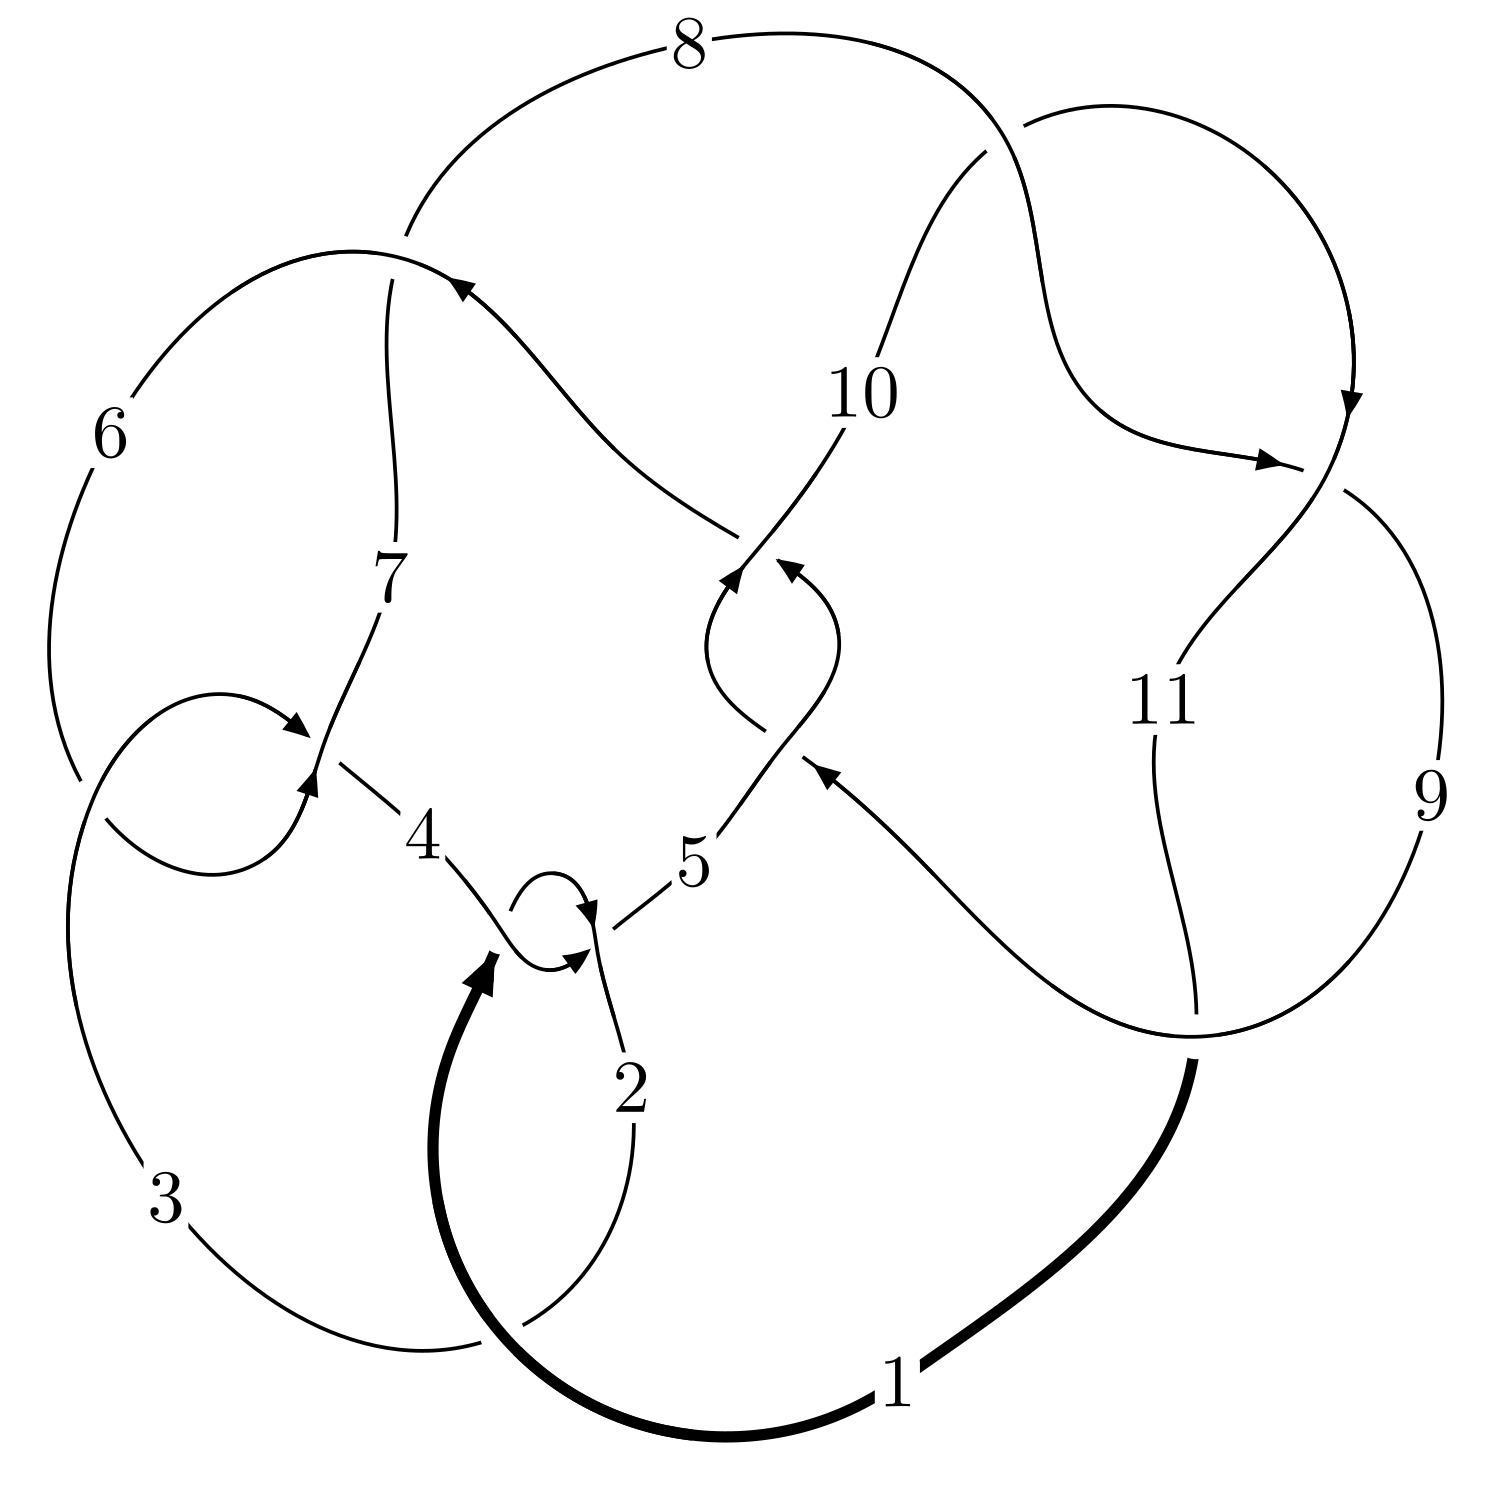
\includegraphics[width=112pt]{../../../GIT/diagram.site/Diagrams/png/271_11a_22.png}\\
\ \ \ A knot diagram\footnotemark}&
\allowdisplaybreaks
\textbf{Linearized knot diagam} \\
\cline{2-2}
 &
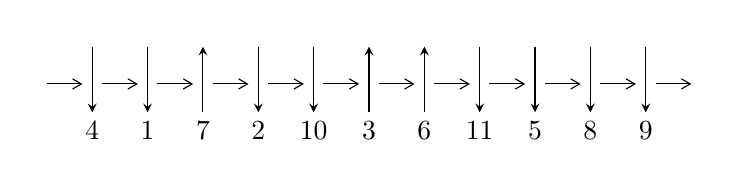
\begin{tikzpicture}[x=20pt, y=17pt]
	% nodes
	\node (C0) at (0, 0) {};
	\node (C1) at (1, 0) {};
	\node (C1U) at (1, +1) {};
	\node (C1D) at (1, -1) {4};

	\node (C2) at (2, 0) {};
	\node (C2U) at (2, +1) {};
	\node (C2D) at (2, -1) {1};

	\node (C3) at (3, 0) {};
	\node (C3U) at (3, +1) {};
	\node (C3D) at (3, -1) {7};

	\node (C4) at (4, 0) {};
	\node (C4U) at (4, +1) {};
	\node (C4D) at (4, -1) {2};

	\node (C5) at (5, 0) {};
	\node (C5U) at (5, +1) {};
	\node (C5D) at (5, -1) {10};

	\node (C6) at (6, 0) {};
	\node (C6U) at (6, +1) {};
	\node (C6D) at (6, -1) {3};

	\node (C7) at (7, 0) {};
	\node (C7U) at (7, +1) {};
	\node (C7D) at (7, -1) {6};

	\node (C8) at (8, 0) {};
	\node (C8U) at (8, +1) {};
	\node (C8D) at (8, -1) {11};

	\node (C9) at (9, 0) {};
	\node (C9U) at (9, +1) {};
	\node (C9D) at (9, -1) {5};

	\node (C10) at (10, 0) {};
	\node (C10U) at (10, +1) {};
	\node (C10D) at (10, -1) {8};

	\node (C11) at (11, 0) {};
	\node (C11U) at (11, +1) {};
	\node (C11D) at (11, -1) {9};
	\node (C12) at (12, 0) {};

	% arrows
	\draw[->,>={angle 60}]
	(C0) edge (C1) (C1) edge (C2) (C2) edge (C3) (C3) edge (C4) (C4) edge (C5) (C5) edge (C6) (C6) edge (C7) (C7) edge (C8) (C8) edge (C9) (C9) edge (C10) (C10) edge (C11) (C11) edge (C12) ;	\draw[->,>=stealth]
	(C1U) edge (C1D) (C2U) edge (C2D) (C3D) edge (C3U) (C4U) edge (C4D) (C5U) edge (C5D) (C6D) edge (C6U) (C7D) edge (C7U) (C8U) edge (C8D) (C9U) edge (C9D) (C10U) edge (C10D) (C11U) edge (C11D) ;
	\end{tikzpicture} \\
\hhline{~~} \\& 
\textbf{Solving Sequence} \\ \cline{2-2} 
 &
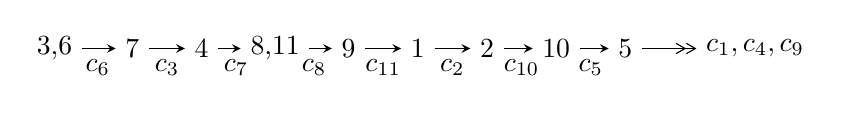
\begin{tikzpicture}[x=25pt, y=7pt]
	% node
	\node (A0) at (-1/8, 0) {3,6};
	\node (A1) at (1, 0) {7};
	\node (A2) at (2, 0) {4};
	\node (A3) at (49/16, 0) {8,11};
	\node (A4) at (33/8, 0) {9};
	\node (A5) at (41/8, 0) {1};
	\node (A6) at (49/8, 0) {2};
	\node (A7) at (57/8, 0) {10};
	\node (A8) at (65/8, 0) {5};
	\node (C1) at (1/2, -1) {$c_{6}$};
	\node (C2) at (3/2, -1) {$c_{3}$};
	\node (C3) at (5/2, -1) {$c_{7}$};
	\node (C4) at (29/8, -1) {$c_{8}$};
	\node (C5) at (37/8, -1) {$c_{11}$};
	\node (C6) at (45/8, -1) {$c_{2}$};
	\node (C7) at (53/8, -1) {$c_{10}$};
	\node (C8) at (61/8, -1) {$c_{5}$};
	\node (A9) at (10, 0) {$c_{1},c_{4},c_{9}$};

	% edge
	\draw[->,>=stealth]	
	(A0) edge (A1) (A1) edge (A2) (A2) edge (A3) (A3) edge (A4) (A4) edge (A5) (A5) edge (A6) (A6) edge (A7) (A7) edge (A8) ;
	\draw[->>,>={angle 60}]	
	(A8) edge (A9);
\end{tikzpicture} \\ 

\end{tabular} \\

\footnotetext{
The image of knot diagram is generated by the software ``\textbf{Draw programme}" developed by Andrew Bartholomew(\url{http://www.layer8.co.uk/maths/draw/index.htm\#Running-draw}), where we modified some parts for our purpose(\url{https://github.com/CATsTAILs/LinksPainter}).
}\phantom \\ \newline 
\centering \textbf{Ideals for irreducible components\footnotemark of $X_{\text{par}}$} 
 
\begin{align*}
I^u_{1}&=\langle 
2.20922\times10^{53} u^{57}+5.38010\times10^{53} u^{56}+\cdots+1.93523\times10^{52} b-1.93917\times10^{54},\\
\phantom{I^u_{1}}&\phantom{= \langle  }8.75242\times10^{53} u^{57}+2.15695\times10^{54} u^{56}+\cdots+3.87047\times10^{52} a-7.51888\times10^{54},\;u^{58}+2 u^{57}+\cdots-20 u+4\rangle \\
I^u_{2}&=\langle 
- u^2+b,\;- u^5+2 u^3+a-2 u,\;u^6+u^5- u^4-2 u^3+u+1\rangle \\
\\
I^v_{1}&=\langle 
a,\;b+v+2,\;v^2+3 v+1\rangle \\
\end{align*}
\raggedright * 3 irreducible components of $\dim_{\mathbb{C}}=0$, with total 66 representations.\\
\footnotetext{All coefficients of polynomials are rational numbers. But the coefficients are sometimes approximated in decimal forms when there is not enough margin.}
\newpage
\renewcommand{\arraystretch}{1}
\centering \section*{I. $I^u_{1}= \langle 2.21\times10^{53} u^{57}+5.38\times10^{53} u^{56}+\cdots+1.94\times10^{52} b-1.94\times10^{54},\;8.75\times10^{53} u^{57}+2.16\times10^{54} u^{56}+\cdots+3.87\times10^{52} a-7.52\times10^{54},\;u^{58}+2 u^{57}+\cdots-20 u+4 \rangle$}
\flushleft \textbf{(i) Arc colorings}\\
\begin{tabular}{m{7pt} m{180pt} m{7pt} m{180pt} }
\flushright $a_{3}=$&$\begin{pmatrix}0\\u\end{pmatrix}$ \\
\flushright $a_{6}=$&$\begin{pmatrix}1\\0\end{pmatrix}$ \\
\flushright $a_{7}=$&$\begin{pmatrix}1\\- u^2\end{pmatrix}$ \\
\flushright $a_{4}=$&$\begin{pmatrix}u\\- u^3+u\end{pmatrix}$ \\
\flushright $a_{8}=$&$\begin{pmatrix}- u^2+1\\- u^2\end{pmatrix}$ \\
\flushright $a_{11}=$&$\begin{pmatrix}-22.6133 u^{57}-55.7283 u^{56}+\cdots-545.664 u+194.263\\-11.4158 u^{57}-27.8007 u^{56}+\cdots-276.503 u+100.203\end{pmatrix}$ \\
\flushright $a_{9}=$&$\begin{pmatrix}-5.51590 u^{57}-13.4288 u^{56}+\cdots-123.425 u+47.3451\\23.7116 u^{57}+58.8709 u^{56}+\cdots+589.977 u-207.708\end{pmatrix}$ \\
\flushright $a_{1}=$&$\begin{pmatrix}-4.78464 u^{57}-12.0436 u^{56}+\cdots-122.072 u+39.9544\\24.1900 u^{57}+59.1862 u^{56}+\cdots+587.084 u-206.905\end{pmatrix}$ \\
\flushright $a_{2}=$&$\begin{pmatrix}-10.8746 u^{57}-27.0241 u^{56}+\cdots-269.732 u+91.6352\\19.4239 u^{57}+47.5510 u^{56}+\cdots+471.075 u-166.426\end{pmatrix}$ \\
\flushright $a_{10}=$&$\begin{pmatrix}-33.5809 u^{57}-82.6520 u^{56}+\cdots-817.229 u+291.314\\-8.47974 u^{57}-20.5966 u^{56}+\cdots-205.705 u+74.9209\end{pmatrix}$ \\
\flushright $a_{5}=$&$\begin{pmatrix}-28.9747 u^{57}-71.2298 u^{56}+\cdots-709.155 u+246.859\\-17.5651 u^{57}-43.1972 u^{56}+\cdots-437.372 u+153.783\end{pmatrix}$\\ \flushright $a_{5}=$&$\begin{pmatrix}-28.9747 u^{57}-71.2298 u^{56}+\cdots-709.155 u+246.859\\-17.5651 u^{57}-43.1972 u^{56}+\cdots-437.372 u+153.783\end{pmatrix}$\\&\end{tabular}
\flushleft \textbf{(ii) Obstruction class $= -1$}\\~\\
\flushleft \textbf{(iii) Cusp Shapes $= 11.5795 u^{57}+27.4881 u^{56}+\cdots+286.625 u-124.569$}\\~\\
\newpage\renewcommand{\arraystretch}{1}
\flushleft \textbf{(iv) u-Polynomials at the component}\newline \\
\begin{tabular}{m{50pt}|m{274pt}}
Crossings & \hspace{64pt}u-Polynomials at each crossing \\
\hline $$\begin{aligned}c_{1},c_{4}\end{aligned}$$&$\begin{aligned}
&u^{58}-4 u^{57}+\cdots-14 u+1
\end{aligned}$\\
\hline $$\begin{aligned}c_{2}\end{aligned}$$&$\begin{aligned}
&u^{58}+32 u^{57}+\cdots+94 u+1
\end{aligned}$\\
\hline $$\begin{aligned}c_{3},c_{6}\end{aligned}$$&$\begin{aligned}
&u^{58}-2 u^{57}+\cdots+20 u+4
\end{aligned}$\\
\hline $$\begin{aligned}c_{5},c_{9}\end{aligned}$$&$\begin{aligned}
&u^{58}+2 u^{57}+\cdots+128 u+64
\end{aligned}$\\
\hline $$\begin{aligned}c_{7}\end{aligned}$$&$\begin{aligned}
&u^{58}-18 u^{57}+\cdots-360 u+16
\end{aligned}$\\
\hline $$\begin{aligned}c_{8},c_{10},c_{11}\end{aligned}$$&$\begin{aligned}
&u^{58}-8 u^{57}+\cdots-4 u+1
\end{aligned}$\\
\hline
\end{tabular}\\~\\
\newpage\renewcommand{\arraystretch}{1}
\flushleft \textbf{(v) Riley Polynomials at the component}\newline \\
\begin{tabular}{m{50pt}|m{274pt}}
Crossings & \hspace{64pt}Riley Polynomials at each crossing \\
\hline $$\begin{aligned}c_{1},c_{4}\end{aligned}$$&$\begin{aligned}
&y^{58}-32 y^{57}+\cdots-94 y+1
\end{aligned}$\\
\hline $$\begin{aligned}c_{2}\end{aligned}$$&$\begin{aligned}
&y^{58}-8 y^{57}+\cdots-7838 y+1
\end{aligned}$\\
\hline $$\begin{aligned}c_{3},c_{6}\end{aligned}$$&$\begin{aligned}
&y^{58}-18 y^{57}+\cdots-360 y+16
\end{aligned}$\\
\hline $$\begin{aligned}c_{5},c_{9}\end{aligned}$$&$\begin{aligned}
&y^{58}-42 y^{57}+\cdots-8192 y+4096
\end{aligned}$\\
\hline $$\begin{aligned}c_{7}\end{aligned}$$&$\begin{aligned}
&y^{58}+42 y^{57}+\cdots-33056 y+256
\end{aligned}$\\
\hline $$\begin{aligned}c_{8},c_{10},c_{11}\end{aligned}$$&$\begin{aligned}
&y^{58}-60 y^{57}+\cdots-36 y+1
\end{aligned}$\\
\hline
\end{tabular}\\~\\
\newpage\flushleft \textbf{(vi) Complex Volumes and Cusp Shapes}
$$\begin{array}{c|c|c}  
\text{Solutions to }I^u_{1}& \I (\text{vol} + \sqrt{-1}CS) & \text{Cusp shape}\\
 \hline 
\begin{aligned}
u &= \phantom{-}0.751278 + 0.687165 I \\
a &= \phantom{-}0.397223 + 0.633477 I \\
b &= \phantom{-}0.489389 + 0.795565 I\end{aligned}
 & -2.18920 + 0.10128 I & -7.14023 + 0. I\phantom{ +0.000000I} \\ \hline\begin{aligned}
u &= \phantom{-}0.751278 - 0.687165 I \\
a &= \phantom{-}0.397223 - 0.633477 I \\
b &= \phantom{-}0.489389 - 0.795565 I\end{aligned}
 & -2.18920 - 0.10128 I & -7.14023 + 0. I\phantom{ +0.000000I} \\ \hline\begin{aligned}
u &= -0.938205 + 0.408426 I \\
a &= \phantom{-}0.231074 + 0.260146 I \\
b &= -0.593325 + 0.623788 I\end{aligned}
 & \phantom{-}1.56893 - 1.49125 I & \phantom{-}1.52605 + 1.85258 I \\ \hline\begin{aligned}
u &= -0.938205 - 0.408426 I \\
a &= \phantom{-}0.231074 - 0.260146 I \\
b &= -0.593325 - 0.623788 I\end{aligned}
 & \phantom{-}1.56893 + 1.49125 I & \phantom{-}1.52605 - 1.85258 I \\ \hline\begin{aligned}
u &= \phantom{-}0.975459\phantom{ +0.000000I} \\
a &= -1.52269\phantom{ +0.000000I} \\
b &= -0.110488\phantom{ +0.000000I}\end{aligned}
 & -8.12166\phantom{ +0.000000I} & -10.1040\phantom{ +0.000000I} \\ \hline\begin{aligned}
u &= -1.025320 + 0.037106 I \\
a &= -0.086100 + 0.547603 I \\
b &= -0.554847 - 0.036376 I\end{aligned}
 & \phantom{-}2.76529 + 0.01343 I & \phantom{-}                -6
1.057430 + 0. 10   I\phantom{ +0.000000I} \\ \hline\begin{aligned}
u &= -1.025320 - 0.037106 I \\
a &= -0.086100 - 0.547603 I \\
b &= -0.554847 + 0.036376 I\end{aligned}
 & \phantom{-}2.76529 - 0.01343 I & \phantom{-}                -6
1.057430 + 0. 10   I\phantom{ +0.000000I} \\ \hline\begin{aligned}
u &= \phantom{-}0.141484 + 1.046590 I \\
a &= \phantom{-}1.95002 - 0.42418 I \\
b &= \phantom{-}0.327448 - 0.475424 I\end{aligned}
 & -6.51259 - 2.28009 I & -10.96046 + 3.19134 I \\ \hline\begin{aligned}
u &= \phantom{-}0.141484 - 1.046590 I \\
a &= \phantom{-}1.95002 + 0.42418 I \\
b &= \phantom{-}0.327448 + 0.475424 I\end{aligned}
 & -6.51259 + 2.28009 I & -10.96046 - 3.19134 I \\ \hline\begin{aligned}
u &= -0.907614 + 0.233881 I \\
a &= \phantom{-}0.452411 + 0.038868 I \\
b &= \phantom{-}1.68026 - 1.11227 I\end{aligned}
 & -1.05945 - 3.12017 I & -5.50127 + 4.47326 I\\
 \hline 
 \end{array}$$\newpage$$\begin{array}{c|c|c}  
\text{Solutions to }I^u_{1}& \I (\text{vol} + \sqrt{-1}CS) & \text{Cusp shape}\\
 \hline 
\begin{aligned}
u &= -0.907614 - 0.233881 I \\
a &= \phantom{-}0.452411 - 0.038868 I \\
b &= \phantom{-}1.68026 + 1.11227 I\end{aligned}
 & -1.05945 + 3.12017 I & -5.50127 - 4.47326 I \\ \hline\begin{aligned}
u &= -0.766366 + 0.768934 I \\
a &= \phantom{-}0.43828 + 2.14321 I \\
b &= -1.37901 + 2.34528 I\end{aligned}
 & -13.34930 - 0.72037 I & -12.98227 + 3.28415 I \\ \hline\begin{aligned}
u &= -0.766366 - 0.768934 I \\
a &= \phantom{-}0.43828 - 2.14321 I \\
b &= -1.37901 - 2.34528 I\end{aligned}
 & -13.34930 + 0.72037 I & -12.98227 - 3.28415 I \\ \hline\begin{aligned}
u &= \phantom{-}1.056160 + 0.263793 I \\
a &= -0.226907 - 0.684770 I \\
b &= -0.294684 - 0.046749 I\end{aligned}
 & \phantom{-}2.08472 + 4.56768 I & \phantom{-0.000000 } 0. - 7.20311 I \\ \hline\begin{aligned}
u &= \phantom{-}1.056160 - 0.263793 I \\
a &= -0.226907 + 0.684770 I \\
b &= -0.294684 + 0.046749 I\end{aligned}
 & \phantom{-}2.08472 - 4.56768 I & \phantom{-0.000000 -}0. + 7.20311 I \\ \hline\begin{aligned}
u &= -0.816044 + 0.752910 I \\
a &= -1.43375 - 0.08308 I \\
b &= -0.202312 - 0.820966 I\end{aligned}
 & -5.71379 - 1.22939 I & \phantom{-0.000000 } 0 \\ \hline\begin{aligned}
u &= -0.816044 - 0.752910 I \\
a &= -1.43375 + 0.08308 I \\
b &= -0.202312 + 0.820966 I\end{aligned}
 & -5.71379 + 1.22939 I & \phantom{-0.000000 } 0 \\ \hline\begin{aligned}
u &= \phantom{-}0.531681 + 0.702789 I \\
a &= \phantom{-}1.041460 - 0.332937 I \\
b &= \phantom{-}0.178506 - 0.656257 I\end{aligned}
 & -2.16889 - 1.07216 I & -4.64986 + 0.67610 I \\ \hline\begin{aligned}
u &= \phantom{-}0.531681 - 0.702789 I \\
a &= \phantom{-}1.041460 + 0.332937 I \\
b &= \phantom{-}0.178506 + 0.656257 I\end{aligned}
 & -2.16889 + 1.07216 I & -4.64986 - 0.67610 I \\ \hline\begin{aligned}
u &= -0.871904 + 0.708903 I \\
a &= -1.62017 - 1.84549 I \\
b &= \phantom{-}0.60927 - 2.97487 I\end{aligned}
 & -3.98695 - 2.71614 I & \phantom{-0.000000 } 0\\
 \hline 
 \end{array}$$\newpage$$\begin{array}{c|c|c}  
\text{Solutions to }I^u_{1}& \I (\text{vol} + \sqrt{-1}CS) & \text{Cusp shape}\\
 \hline 
\begin{aligned}
u &= -0.871904 - 0.708903 I \\
a &= -1.62017 + 1.84549 I \\
b &= \phantom{-}0.60927 + 2.97487 I\end{aligned}
 & -3.98695 + 2.71614 I & \phantom{-0.000000 } 0 \\ \hline\begin{aligned}
u &= \phantom{-}0.646879 + 0.932661 I \\
a &= \phantom{-}1.23701 - 2.00036 I \\
b &= -0.50044 - 2.21446 I\end{aligned}
 & -9.34785 - 3.11893 I & \phantom{-0.000000 } 0 \\ \hline\begin{aligned}
u &= \phantom{-}0.646879 - 0.932661 I \\
a &= \phantom{-}1.23701 + 2.00036 I \\
b &= -0.50044 + 2.21446 I\end{aligned}
 & -9.34785 + 3.11893 I & \phantom{-0.000000 } 0 \\ \hline\begin{aligned}
u &= \phantom{-}0.786683 + 0.828955 I \\
a &= -2.61581 + 2.03754 I \\
b &= -0.16255 + 3.14290 I\end{aligned}
 & -7.78075 - 1.40297 I & \phantom{-0.000000 } 0 \\ \hline\begin{aligned}
u &= \phantom{-}0.786683 - 0.828955 I \\
a &= -2.61581 - 2.03754 I \\
b &= -0.16255 - 3.14290 I\end{aligned}
 & -7.78075 + 1.40297 I & \phantom{-0.000000 } 0 \\ \hline\begin{aligned}
u &= -0.733599 + 0.883254 I \\
a &= \phantom{-}0.012106 - 0.387354 I \\
b &= \phantom{-}0.049160 - 0.756342 I\end{aligned}
 & -5.55187 + 4.00580 I & \phantom{-0.000000 } 0 \\ \hline\begin{aligned}
u &= -0.733599 - 0.883254 I \\
a &= \phantom{-}0.012106 + 0.387354 I \\
b &= \phantom{-}0.049160 + 0.756342 I\end{aligned}
 & -5.55187 - 4.00580 I & \phantom{-0.000000 } 0 \\ \hline\begin{aligned}
u &= \phantom{-}0.844172 + 0.085017 I \\
a &= \phantom{-}0.986920 + 0.702481 I \\
b &= \phantom{-}1.49717 - 0.05675 I\end{aligned}
 & -0.629418 + 0.623631 I & -5.36343 - 3.54196 I \\ \hline\begin{aligned}
u &= \phantom{-}0.844172 - 0.085017 I \\
a &= \phantom{-}0.986920 - 0.702481 I \\
b &= \phantom{-}1.49717 + 0.05675 I\end{aligned}
 & -0.629418 - 0.623631 I & -5.36343 + 3.54196 I \\ \hline\begin{aligned}
u &= \phantom{-}0.959680 + 0.687124 I \\
a &= -0.783612 + 0.016039 I \\
b &= \phantom{-}0.095816 + 0.597900 I\end{aligned}
 & -1.54879 + 5.22529 I & \phantom{-0.000000 } 0\\
 \hline 
 \end{array}$$\newpage$$\begin{array}{c|c|c}  
\text{Solutions to }I^u_{1}& \I (\text{vol} + \sqrt{-1}CS) & \text{Cusp shape}\\
 \hline 
\begin{aligned}
u &= \phantom{-}0.959680 - 0.687124 I \\
a &= -0.783612 - 0.016039 I \\
b &= \phantom{-}0.095816 - 0.597900 I\end{aligned}
 & -1.54879 - 5.22529 I & \phantom{-0.000000 } 0 \\ \hline\begin{aligned}
u &= -0.925912 + 0.732408 I \\
a &= \phantom{-}0.191499 - 1.003200 I \\
b &= \phantom{-}0.468873 - 1.260970 I\end{aligned}
 & -5.37580 - 4.41103 I & \phantom{-0.000000 } 0 \\ \hline\begin{aligned}
u &= -0.925912 - 0.732408 I \\
a &= \phantom{-}0.191499 + 1.003200 I \\
b &= \phantom{-}0.468873 + 1.260970 I\end{aligned}
 & -5.37580 + 4.41103 I & \phantom{-0.000000 } 0 \\ \hline\begin{aligned}
u &= \phantom{-}1.032960 + 0.608744 I \\
a &= \phantom{-}0.192674 - 0.762403 I \\
b &= -0.660062 - 1.066530 I\end{aligned}
 & -0.69171 + 6.13139 I & \phantom{-0.000000 } 0 \\ \hline\begin{aligned}
u &= \phantom{-}1.032960 - 0.608744 I \\
a &= \phantom{-}0.192674 + 0.762403 I \\
b &= -0.660062 + 1.066530 I\end{aligned}
 & -0.69171 - 6.13139 I & \phantom{-0.000000 } 0 \\ \hline\begin{aligned}
u &= -0.970390 + 0.723923 I \\
a &= \phantom{-}1.94328 + 0.72453 I \\
b &= \phantom{-}0.47039 + 2.60152 I\end{aligned}
 & -12.71920 - 4.94560 I & \phantom{-0.000000 } 0 \\ \hline\begin{aligned}
u &= -0.970390 - 0.723923 I \\
a &= \phantom{-}1.94328 - 0.72453 I \\
b &= \phantom{-}0.47039 - 2.60152 I\end{aligned}
 & -12.71920 + 4.94560 I & \phantom{-0.000000 } 0 \\ \hline\begin{aligned}
u &= \phantom{-}0.971435 + 0.767699 I \\
a &= -1.37396 + 2.61714 I \\
b &= \phantom{-}0.85784 + 3.57871 I\end{aligned}
 & -7.20694 + 7.37757 I & \phantom{-0.000000 } 0 \\ \hline\begin{aligned}
u &= \phantom{-}0.971435 - 0.767699 I \\
a &= -1.37396 - 2.61714 I \\
b &= \phantom{-}0.85784 - 3.57871 I\end{aligned}
 & -7.20694 - 7.37757 I & \phantom{-0.000000 } 0 \\ \hline\begin{aligned}
u &= -0.749801 + 1.013650 I \\
a &= \phantom{-}1.42076 + 2.51991 I \\
b &= -0.31957 + 2.79288 I\end{aligned}
 & -12.3578 + 7.9362 I & \phantom{-0.000000 } 0\\
 \hline 
 \end{array}$$\newpage$$\begin{array}{c|c|c}  
\text{Solutions to }I^u_{1}& \I (\text{vol} + \sqrt{-1}CS) & \text{Cusp shape}\\
 \hline 
\begin{aligned}
u &= -0.749801 - 1.013650 I \\
a &= \phantom{-}1.42076 - 2.51991 I \\
b &= -0.31957 - 2.79288 I\end{aligned}
 & -12.3578 - 7.9362 I & \phantom{-0.000000 } 0 \\ \hline\begin{aligned}
u &= -1.260080 + 0.222648 I \\
a &= -1.043850 + 0.235063 I \\
b &= -1.069910 + 0.809848 I\end{aligned}
 & -1.33556 - 1.90763 I & \phantom{-0.000000 } 0 \\ \hline\begin{aligned}
u &= -1.260080 - 0.222648 I \\
a &= -1.043850 - 0.235063 I \\
b &= -1.069910 - 0.809848 I\end{aligned}
 & -1.33556 + 1.90763 I & \phantom{-0.000000 } 0 \\ \hline\begin{aligned}
u &= -1.021410 + 0.771092 I \\
a &= -0.608745 - 0.376035 I \\
b &= \phantom{-}0.332932 - 0.745316 I\end{aligned}
 & -4.65387 - 10.14070 I & \phantom{-0.000000 } 0 \\ \hline\begin{aligned}
u &= -1.021410 - 0.771092 I \\
a &= -0.608745 + 0.376035 I \\
b &= \phantom{-}0.332932 + 0.745316 I\end{aligned}
 & -4.65387 + 10.14070 I & \phantom{-0.000000 } 0 \\ \hline\begin{aligned}
u &= \phantom{-}0.117607 + 0.695097 I \\
a &= \phantom{-}0.967277 - 0.036072 I \\
b &= \phantom{-}0.433545 + 0.151204 I\end{aligned}
 & -1.14303 - 1.20148 I & -5.78859 + 5.55533 I \\ \hline\begin{aligned}
u &= \phantom{-}0.117607 - 0.695097 I \\
a &= \phantom{-}0.967277 + 0.036072 I \\
b &= \phantom{-}0.433545 - 0.151204 I\end{aligned}
 & -1.14303 + 1.20148 I & -5.78859 - 5.55533 I \\ \hline\begin{aligned}
u &= \phantom{-}1.249040 + 0.401910 I \\
a &= -0.605347 - 0.578787 I \\
b &= -0.98878 - 1.48797 I\end{aligned}
 & -2.57248 + 7.45358 I & \phantom{-0.000000 } 0 \\ \hline\begin{aligned}
u &= \phantom{-}1.249040 - 0.401910 I \\
a &= -0.605347 + 0.578787 I \\
b &= -0.98878 + 1.48797 I\end{aligned}
 & -2.57248 - 7.45358 I & \phantom{-0.000000 } 0 \\ \hline\begin{aligned}
u &= \phantom{-}1.073950 + 0.758891 I \\
a &= \phantom{-}1.50409 - 1.45263 I \\
b &= \phantom{-}0.04645 - 2.93251 I\end{aligned}
 & -8.03060 + 9.32855 I & \phantom{-0.000000 } 0\\
 \hline 
 \end{array}$$\newpage$$\begin{array}{c|c|c}  
\text{Solutions to }I^u_{1}& \I (\text{vol} + \sqrt{-1}CS) & \text{Cusp shape}\\
 \hline 
\begin{aligned}
u &= \phantom{-}1.073950 - 0.758891 I \\
a &= \phantom{-}1.50409 + 1.45263 I \\
b &= \phantom{-}0.04645 + 2.93251 I\end{aligned}
 & -8.03060 - 9.32855 I & \phantom{-0.000000 } 0 \\ \hline\begin{aligned}
u &= -1.082250 + 0.829438 I \\
a &= \phantom{-}1.77158 + 1.93052 I \\
b &= \phantom{-}0.11809 + 3.30285 I\end{aligned}
 & -11.2723 - 14.6533 I & \phantom{-0.000000 } 0 \\ \hline\begin{aligned}
u &= -1.082250 - 0.829438 I \\
a &= \phantom{-}1.77158 - 1.93052 I \\
b &= \phantom{-}0.11809 - 3.30285 I\end{aligned}
 & -11.2723 + 14.6533 I & \phantom{-0.000000 } 0 \\ \hline\begin{aligned}
u &= -0.209439 + 0.468075 I \\
a &= -5.64495 + 2.38701 I \\
b &= -0.441139 - 0.581010 I\end{aligned}
 & -3.24157 + 0.49714 I & -10.0374 + 15.0443 I \\ \hline\begin{aligned}
u &= -0.209439 - 0.468075 I \\
a &= -5.64495 - 2.38701 I \\
b &= -0.441139 + 0.581010 I\end{aligned}
 & -3.24157 - 0.49714 I & -10.0374 - 15.0443 I \\ \hline\begin{aligned}
u &= \phantom{-}0.471619\phantom{ +0.000000I} \\
a &= \phantom{-}3.18461\phantom{ +0.000000I} \\
b &= -0.472950\phantom{ +0.000000I}\end{aligned}
 & -2.28699\phantom{ +0.000000I} & \phantom{-}3.94780\phantom{ +0.000000I} \\ \hline\begin{aligned}
u &= \phantom{-}0.459325\phantom{ +0.000000I} \\
a &= -0.198494\phantom{ +0.000000I} \\
b &= -2.04304\phantom{ +0.000000I}\end{aligned}
 & -10.2057\phantom{ +0.000000I} & \phantom{-}4.64730\phantom{ +0.000000I} \\ \hline\begin{aligned}
u &= \phantom{-}0.324240\phantom{ +0.000000I} \\
a &= \phantom{-}1.64764\phantom{ +0.000000I} \\
b &= \phantom{-}0.649452\phantom{ +0.000000I}\end{aligned}
 & -1.11333\phantom{ +0.000000I} & -8.96690\phantom{ +0.000000I}\\
 \hline 
 \end{array}$$\newpage\newpage\renewcommand{\arraystretch}{1}
\centering \section*{II. $I^u_{2}= \langle - u^2+b,\;- u^5+2 u^3+a-2 u,\;u^6+u^5- u^4-2 u^3+u+1 \rangle$}
\flushleft \textbf{(i) Arc colorings}\\
\begin{tabular}{m{7pt} m{180pt} m{7pt} m{180pt} }
\flushright $a_{3}=$&$\begin{pmatrix}0\\u\end{pmatrix}$ \\
\flushright $a_{6}=$&$\begin{pmatrix}1\\0\end{pmatrix}$ \\
\flushright $a_{7}=$&$\begin{pmatrix}1\\- u^2\end{pmatrix}$ \\
\flushright $a_{4}=$&$\begin{pmatrix}u\\- u^3+u\end{pmatrix}$ \\
\flushright $a_{8}=$&$\begin{pmatrix}- u^2+1\\- u^2\end{pmatrix}$ \\
\flushright $a_{11}=$&$\begin{pmatrix}u^5-2 u^3+2 u\\u^2\end{pmatrix}$ \\
\flushright $a_{9}=$&$\begin{pmatrix}u^5-2 u^3- u^2+2 u+1\\0\end{pmatrix}$ \\
\flushright $a_{1}=$&$\begin{pmatrix}u^2-1\\u^2\end{pmatrix}$ \\
\flushright $a_{2}=$&$\begin{pmatrix}u^5-2 u^3+u\\u^5- u^3+u\end{pmatrix}$ \\
\flushright $a_{10}=$&$\begin{pmatrix}u^5-2 u^3- u^2+2 u+1\\0\end{pmatrix}$ \\
\flushright $a_{5}=$&$\begin{pmatrix}1\\0\end{pmatrix}$\\ \flushright $a_{5}=$&$\begin{pmatrix}1\\0\end{pmatrix}$\\&\end{tabular}
\flushleft \textbf{(ii) Obstruction class $= 1$}\\~\\
\flushleft \textbf{(iii) Cusp Shapes $= - u^5-5 u^4+u^3+7 u^2+4 u-12$}\\~\\
\newpage\renewcommand{\arraystretch}{1}
\flushleft \textbf{(iv) u-Polynomials at the component}\newline \\
\begin{tabular}{m{50pt}|m{274pt}}
Crossings & \hspace{64pt}u-Polynomials at each crossing \\
\hline $$\begin{aligned}c_{1},c_{6}\end{aligned}$$&$\begin{aligned}
&u^6+u^5- u^4-2 u^3+u+1
\end{aligned}$\\
\hline $$\begin{aligned}c_{2}\end{aligned}$$&$\begin{aligned}
&u^6+3 u^5+5 u^4+4 u^3+2 u^2+u+1
\end{aligned}$\\
\hline $$\begin{aligned}c_{3},c_{4}\end{aligned}$$&$\begin{aligned}
&u^6- u^5- u^4+2 u^3- u+1
\end{aligned}$\\
\hline $$\begin{aligned}c_{5},c_{9}\end{aligned}$$&$\begin{aligned}
&u^6
\end{aligned}$\\
\hline $$\begin{aligned}c_{7}\end{aligned}$$&$\begin{aligned}
&u^6-3 u^5+5 u^4-4 u^3+2 u^2- u+1
\end{aligned}$\\
\hline $$\begin{aligned}c_{8}\end{aligned}$$&$\begin{aligned}
&(u-1)^6
\end{aligned}$\\
\hline $$\begin{aligned}c_{10},c_{11}\end{aligned}$$&$\begin{aligned}
&(u+1)^6
\end{aligned}$\\
\hline
\end{tabular}\\~\\
\newpage\renewcommand{\arraystretch}{1}
\flushleft \textbf{(v) Riley Polynomials at the component}\newline \\
\begin{tabular}{m{50pt}|m{274pt}}
Crossings & \hspace{64pt}Riley Polynomials at each crossing \\
\hline $$\begin{aligned}c_{1},c_{3},c_{4}\\c_{6}\end{aligned}$$&$\begin{aligned}
&y^6-3 y^5+5 y^4-4 y^3+2 y^2- y+1
\end{aligned}$\\
\hline $$\begin{aligned}c_{2},c_{7}\end{aligned}$$&$\begin{aligned}
&y^6+y^5+5 y^4+6 y^2+3 y+1
\end{aligned}$\\
\hline $$\begin{aligned}c_{5},c_{9}\end{aligned}$$&$\begin{aligned}
&y^6
\end{aligned}$\\
\hline $$\begin{aligned}c_{8},c_{10},c_{11}\end{aligned}$$&$\begin{aligned}
&(y-1)^6
\end{aligned}$\\
\hline
\end{tabular}\\~\\
\newpage\flushleft \textbf{(vi) Complex Volumes and Cusp Shapes}
$$\begin{array}{c|c|c}  
\text{Solutions to }I^u_{2}& \I (\text{vol} + \sqrt{-1}CS) & \text{Cusp shape}\\
 \hline 
\begin{aligned}
u &= \phantom{-}1.002190 + 0.295542 I \\
a &= \phantom{-}0.686453 + 0.095369 I \\
b &= \phantom{-}0.917045 + 0.592379 I\end{aligned}
 & \phantom{-}0.245672 + 0.924305 I & -3.44826 - 0.47256 I \\ \hline\begin{aligned}
u &= \phantom{-}1.002190 - 0.295542 I \\
a &= \phantom{-}0.686453 - 0.095369 I \\
b &= \phantom{-}0.917045 - 0.592379 I\end{aligned}
 & \phantom{-}0.245672 - 0.924305 I & -3.44826 + 0.47256 I \\ \hline\begin{aligned}
u &= -0.428243 + 0.664531 I \\
a &= -1.91924 + 0.88792 I \\
b &= -0.258209 - 0.569162 I\end{aligned}
 & -3.53554 + 0.92430 I & -13.66012 - 2.42665 I \\ \hline\begin{aligned}
u &= -0.428243 - 0.664531 I \\
a &= -1.91924 - 0.88792 I \\
b &= -0.258209 + 0.569162 I\end{aligned}
 & -3.53554 - 0.92430 I & -13.66012 + 2.42665 I \\ \hline\begin{aligned}
u &= -1.073950 + 0.558752 I \\
a &= \phantom{-}0.232786 - 0.641391 I \\
b &= \phantom{-}0.84116 - 1.20014 I\end{aligned}
 & -1.64493 - 5.69302 I & -8.89162 + 3.92918 I \\ \hline\begin{aligned}
u &= -1.073950 - 0.558752 I \\
a &= \phantom{-}0.232786 + 0.641391 I \\
b &= \phantom{-}0.84116 + 1.20014 I\end{aligned}
 & -1.64493 + 5.69302 I & -8.89162 - 3.92918 I\\
 \hline 
 \end{array}$$\newpage\newpage\renewcommand{\arraystretch}{1}
\centering \section*{III. $I^v_{1}= \langle a,\;b+v+2,\;v^2+3 v+1 \rangle$}
\flushleft \textbf{(i) Arc colorings}\\
\begin{tabular}{m{7pt} m{180pt} m{7pt} m{180pt} }
\flushright $a_{3}=$&$\begin{pmatrix}v\\0\end{pmatrix}$ \\
\flushright $a_{6}=$&$\begin{pmatrix}1\\0\end{pmatrix}$ \\
\flushright $a_{7}=$&$\begin{pmatrix}1\\0\end{pmatrix}$ \\
\flushright $a_{4}=$&$\begin{pmatrix}v\\0\end{pmatrix}$ \\
\flushright $a_{8}=$&$\begin{pmatrix}1\\0\end{pmatrix}$ \\
\flushright $a_{11}=$&$\begin{pmatrix}0\\- v-2\end{pmatrix}$ \\
\flushright $a_{9}=$&$\begin{pmatrix}1\\v+3\end{pmatrix}$ \\
\flushright $a_{1}=$&$\begin{pmatrix}v+2\\v+3\end{pmatrix}$ \\
\flushright $a_{2}=$&$\begin{pmatrix}2 v+2\\v+3\end{pmatrix}$ \\
\flushright $a_{10}=$&$\begin{pmatrix}- v-2\\- v-2\end{pmatrix}$ \\
\flushright $a_{5}=$&$\begin{pmatrix}- v-2\\- v-3\end{pmatrix}$\\ \flushright $a_{5}=$&$\begin{pmatrix}- v-2\\- v-3\end{pmatrix}$\\&\end{tabular}
\flushleft \textbf{(ii) Obstruction class $= 1$}\\~\\
\flushleft \textbf{(iii) Cusp Shapes $= -21$}\\~\\
\newpage\renewcommand{\arraystretch}{1}
\flushleft \textbf{(iv) u-Polynomials at the component}\newline \\
\begin{tabular}{m{50pt}|m{274pt}}
Crossings & \hspace{64pt}u-Polynomials at each crossing \\
\hline $$\begin{aligned}c_{1}\end{aligned}$$&$\begin{aligned}
&(u-1)^2
\end{aligned}$\\
\hline $$\begin{aligned}c_{2},c_{4}\end{aligned}$$&$\begin{aligned}
&(u+1)^2
\end{aligned}$\\
\hline $$\begin{aligned}c_{3},c_{6},c_{7}\end{aligned}$$&$\begin{aligned}
&u^2
\end{aligned}$\\
\hline $$\begin{aligned}c_{5},c_{8}\end{aligned}$$&$\begin{aligned}
&u^2+u-1
\end{aligned}$\\
\hline $$\begin{aligned}c_{9},c_{10},c_{11}\end{aligned}$$&$\begin{aligned}
&u^2- u-1
\end{aligned}$\\
\hline
\end{tabular}\\~\\
\newpage\renewcommand{\arraystretch}{1}
\flushleft \textbf{(v) Riley Polynomials at the component}\newline \\
\begin{tabular}{m{50pt}|m{274pt}}
Crossings & \hspace{64pt}Riley Polynomials at each crossing \\
\hline $$\begin{aligned}c_{1},c_{2},c_{4}\end{aligned}$$&$\begin{aligned}
&(y-1)^2
\end{aligned}$\\
\hline $$\begin{aligned}c_{3},c_{6},c_{7}\end{aligned}$$&$\begin{aligned}
&y^2
\end{aligned}$\\
\hline $$\begin{aligned}c_{5},c_{8},c_{9}\\c_{10},c_{11}\end{aligned}$$&$\begin{aligned}
&y^2-3 y+1
\end{aligned}$\\
\hline
\end{tabular}\\~\\
\newpage\flushleft \textbf{(vi) Complex Volumes and Cusp Shapes}
$$\begin{array}{c|c|c}  
\text{Solutions to }I^v_{1}& \I (\text{vol} + \sqrt{-1}CS) & \text{Cusp shape}\\
 \hline 
\begin{aligned}
v &= -0.381966\phantom{ +0.000000I} \\
a &= \phantom{-0.000000 } 0 \\
b &= -1.61803\phantom{ +0.000000I}\end{aligned}
 & -10.5276\phantom{ +0.000000I} & -21.0000\phantom{ +0.000000I} \\ \hline\begin{aligned}
v &= -2.61803\phantom{ +0.000000I} \\
a &= \phantom{-0.000000 } 0 \\
b &= \phantom{-}0.618034\phantom{ +0.000000I}\end{aligned}
 & -2.63189\phantom{ +0.000000I} & -21.0000\phantom{ +0.000000I}\\
 \hline 
 \end{array}$$\newpage
\newpage\renewcommand{\arraystretch}{1}
\centering \section*{ IV. u-Polynomials}
\begin{tabular}{m{50pt}|m{274pt}}
Crossings & \hspace{64pt}u-Polynomials at each crossing \\
\hline $$\begin{aligned}c_{1}\end{aligned}$$&$\begin{aligned}
&((u-1)^2)(u^6+u^5+\cdots+u+1)(u^{58}-4 u^{57}+\cdots-14 u+1)
\end{aligned}$\\
\hline $$\begin{aligned}c_{2}\end{aligned}$$&$\begin{aligned}
&(u+1)^2(u^6+3 u^5+5 u^4+4 u^3+2 u^2+u+1)\\
&\cdot(u^{58}+32 u^{57}+\cdots+94 u+1)
\end{aligned}$\\
\hline $$\begin{aligned}c_{3}\end{aligned}$$&$\begin{aligned}
&u^2(u^6- u^5+\cdots- u+1)(u^{58}-2 u^{57}+\cdots+20 u+4)
\end{aligned}$\\
\hline $$\begin{aligned}c_{4}\end{aligned}$$&$\begin{aligned}
&((u+1)^2)(u^6- u^5+\cdots- u+1)(u^{58}-4 u^{57}+\cdots-14 u+1)
\end{aligned}$\\
\hline $$\begin{aligned}c_{5}\end{aligned}$$&$\begin{aligned}
&u^6(u^2+u-1)(u^{58}+2 u^{57}+\cdots+128 u+64)
\end{aligned}$\\
\hline $$\begin{aligned}c_{6}\end{aligned}$$&$\begin{aligned}
&u^2(u^6+u^5+\cdots+u+1)(u^{58}-2 u^{57}+\cdots+20 u+4)
\end{aligned}$\\
\hline $$\begin{aligned}c_{7}\end{aligned}$$&$\begin{aligned}
&u^2(u^6-3 u^5+\cdots- u+1)(u^{58}-18 u^{57}+\cdots-360 u+16)
\end{aligned}$\\
\hline $$\begin{aligned}c_{8}\end{aligned}$$&$\begin{aligned}
&((u-1)^6)(u^2+u-1)(u^{58}-8 u^{57}+\cdots-4 u+1)
\end{aligned}$\\
\hline $$\begin{aligned}c_{9}\end{aligned}$$&$\begin{aligned}
&u^6(u^2- u-1)(u^{58}+2 u^{57}+\cdots+128 u+64)
\end{aligned}$\\
\hline $$\begin{aligned}c_{10},c_{11}\end{aligned}$$&$\begin{aligned}
&((u+1)^6)(u^2- u-1)(u^{58}-8 u^{57}+\cdots-4 u+1)
\end{aligned}$\\
\hline
\end{tabular}\newpage\renewcommand{\arraystretch}{1}
\centering \section*{ V. Riley Polynomials}
\begin{tabular}{m{50pt}|m{274pt}}
Crossings & \hspace{64pt}Riley Polynomials at each crossing \\
\hline $$\begin{aligned}c_{1},c_{4}\end{aligned}$$&$\begin{aligned}
&(y-1)^2(y^6-3 y^5+5 y^4-4 y^3+2 y^2- y+1)\\
&\cdot(y^{58}-32 y^{57}+\cdots-94 y+1)
\end{aligned}$\\
\hline $$\begin{aligned}c_{2}\end{aligned}$$&$\begin{aligned}
&((y-1)^2)(y^6+y^5+\cdots+3 y+1)(y^{58}-8 y^{57}+\cdots-7838 y+1)
\end{aligned}$\\
\hline $$\begin{aligned}c_{3},c_{6}\end{aligned}$$&$\begin{aligned}
&y^2(y^6-3 y^5+\cdots- y+1)(y^{58}-18 y^{57}+\cdots-360 y+16)
\end{aligned}$\\
\hline $$\begin{aligned}c_{5},c_{9}\end{aligned}$$&$\begin{aligned}
&y^6(y^2-3 y+1)(y^{58}-42 y^{57}+\cdots-8192 y+4096)
\end{aligned}$\\
\hline $$\begin{aligned}c_{7}\end{aligned}$$&$\begin{aligned}
&y^2(y^6+y^5+\cdots+3 y+1)(y^{58}+42 y^{57}+\cdots-33056 y+256)
\end{aligned}$\\
\hline $$\begin{aligned}c_{8},c_{10},c_{11}\end{aligned}$$&$\begin{aligned}
&((y-1)^6)(y^2-3 y+1)(y^{58}-60 y^{57}+\cdots-36 y+1)
\end{aligned}$\\
\hline
\end{tabular}
\vskip 2pc
\end{document}